
\begin{figure}[!ht]
	\centering
	\includegraphics[width=0.7\textwidth]{main.png}                
	\caption{Moodle Main page}
	\hspace{-1.5em}
\end{figure}\\


\begin{figure}[!ht]
	\centering
	\includegraphics[width=0.7\textwidth]{images/login.png}                
	\caption{Moodle login page}
	\hspace{-1.5em}
\end{figure}
\newpage

\begin{figure}[!ht]
	\centering
	\includegraphics[width=0.7\textwidth]{images/vpl.png}                
	\caption{Online Compilation Module}
	\hspace{-1.5em}
\end{figure}

\begin{figure}[!ht]
	\centering
	\includegraphics[width=0.7\textwidth]{images/runvpl.png}                
	\caption{Running Programs with VPL}
	\hspace{-1.5em}
\end{figure}
\newpage
 \begin{figure}[!ht]
 	\centering
 	\includegraphics[width=0.7\textwidth]{images/output.png}                
 	\caption{VPl Output}
 	\hspace{-1.5em}
 \end{figure}
 
  \begin{figure}[!ht]
  	\centering
  	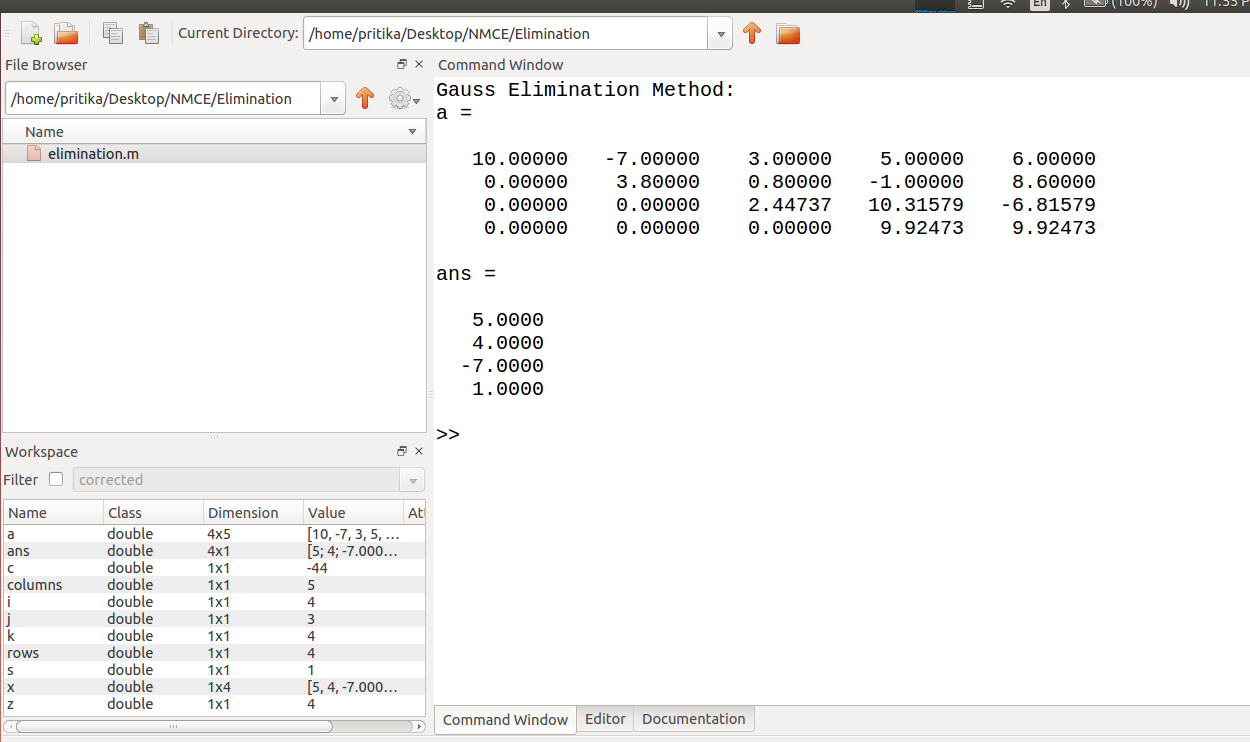
\includegraphics[width=0.7\textwidth]{images/Elimination.png}                
  	\caption{Elimination method }
  	\hspace{-1.5em}
  \end{figure}
  
  \newpage
  Weboctave is a web interface to octave:\\
  \begin{figure}[!ht]
  	\centering
  	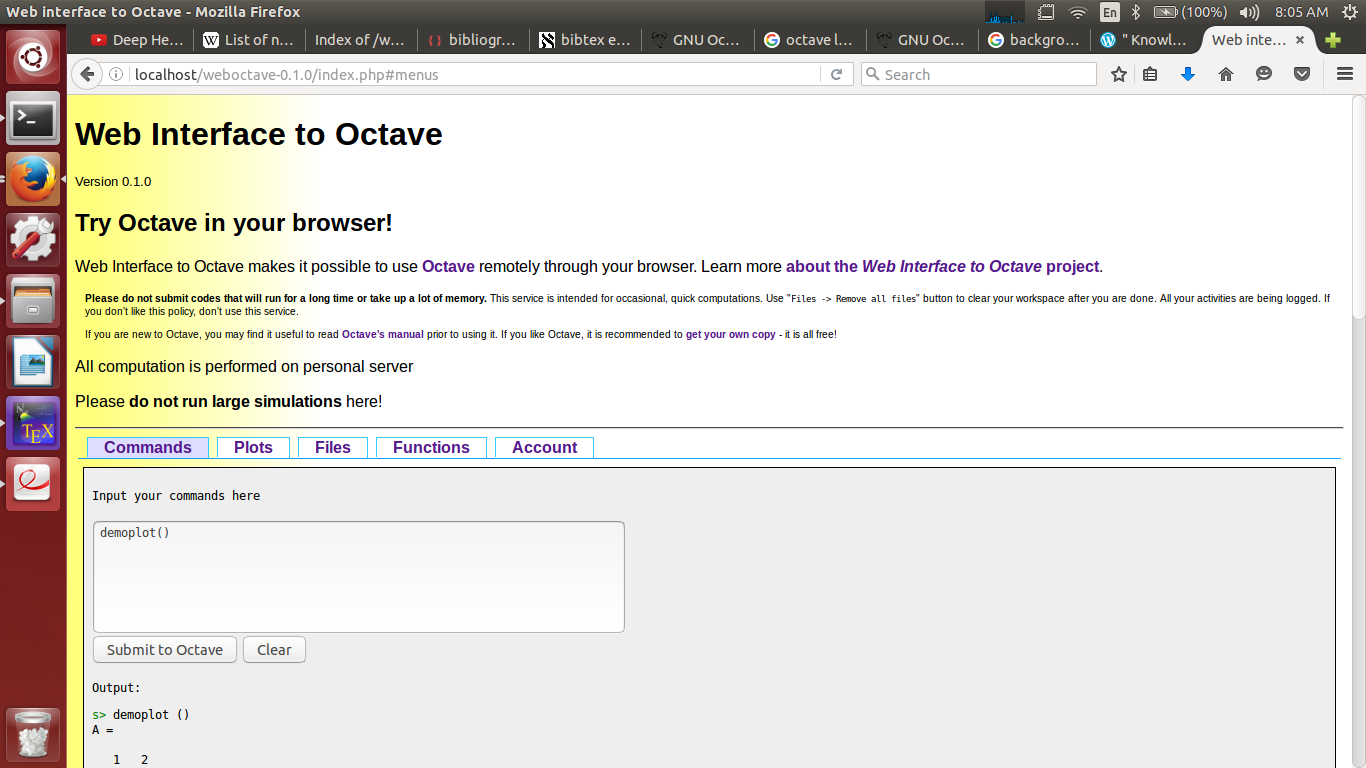
\includegraphics[width=0.7\textwidth]{images/interface.png}                
  	\caption{Weboctave Interface}
  	\hspace{-1.5em}
  \end{figure}
  

\noindent \textbf { The first query with which a user is greeted is:}\\

\noindent function demoplot()\\
A = [1,2;3,4]\\
eig(A)\\
y = x = linspace(0,10);
[X,Y] = meshgrid(x,y);\\
mesh(X,Y,sin(X).*cos(Y).*X);\\
endfunction\\

And it's result can be seen by: 

 \begin{figure}[!ht]
 	\centering
 	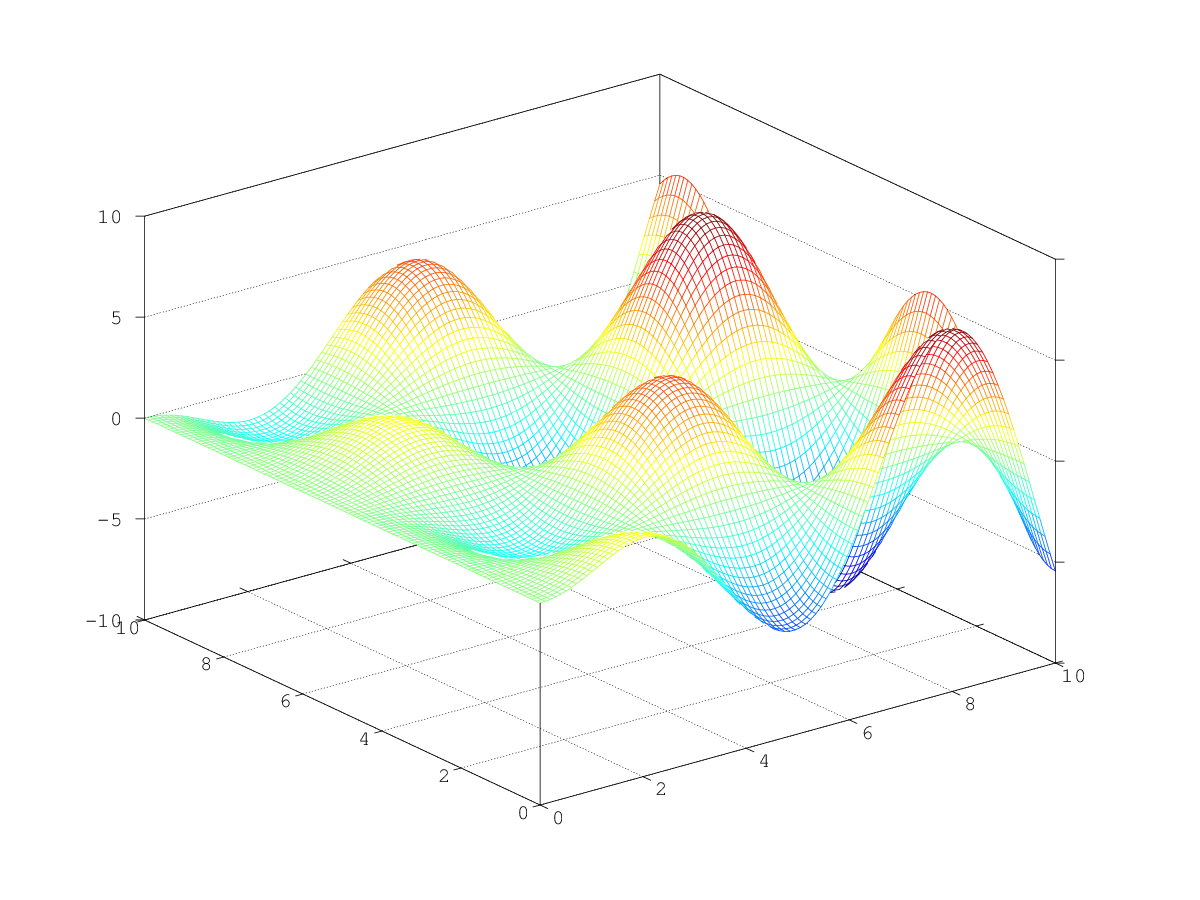
\includegraphics[width=0.7\textwidth]{images/plot1.png}                
 	\caption{Mesh}
 	\hspace{-1.5em}
 \end{figure}
 
 The plots obtained can be downloaded:\\
 \begin{figure}[!ht]
 	\centering
 	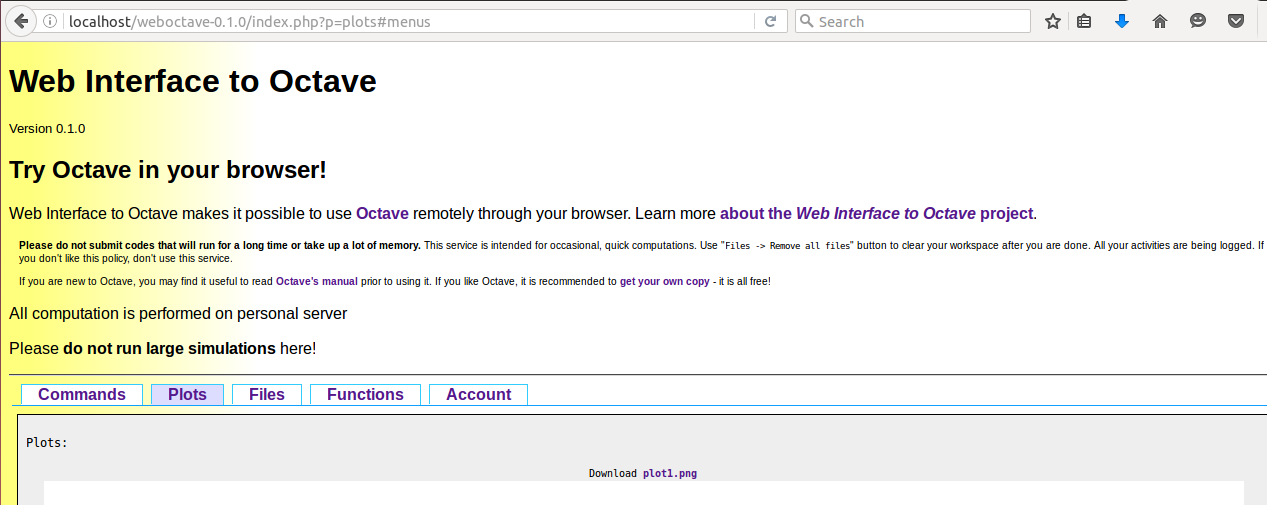
\includegraphics[width=0.7\textwidth]{images/download.png}                
 	\caption{Mesh}
 	\hspace{-1.5em}
 \end{figure}
 \newpage
 User can create his/her account:
 \begin{figure}[!ht]
 	\centering
 	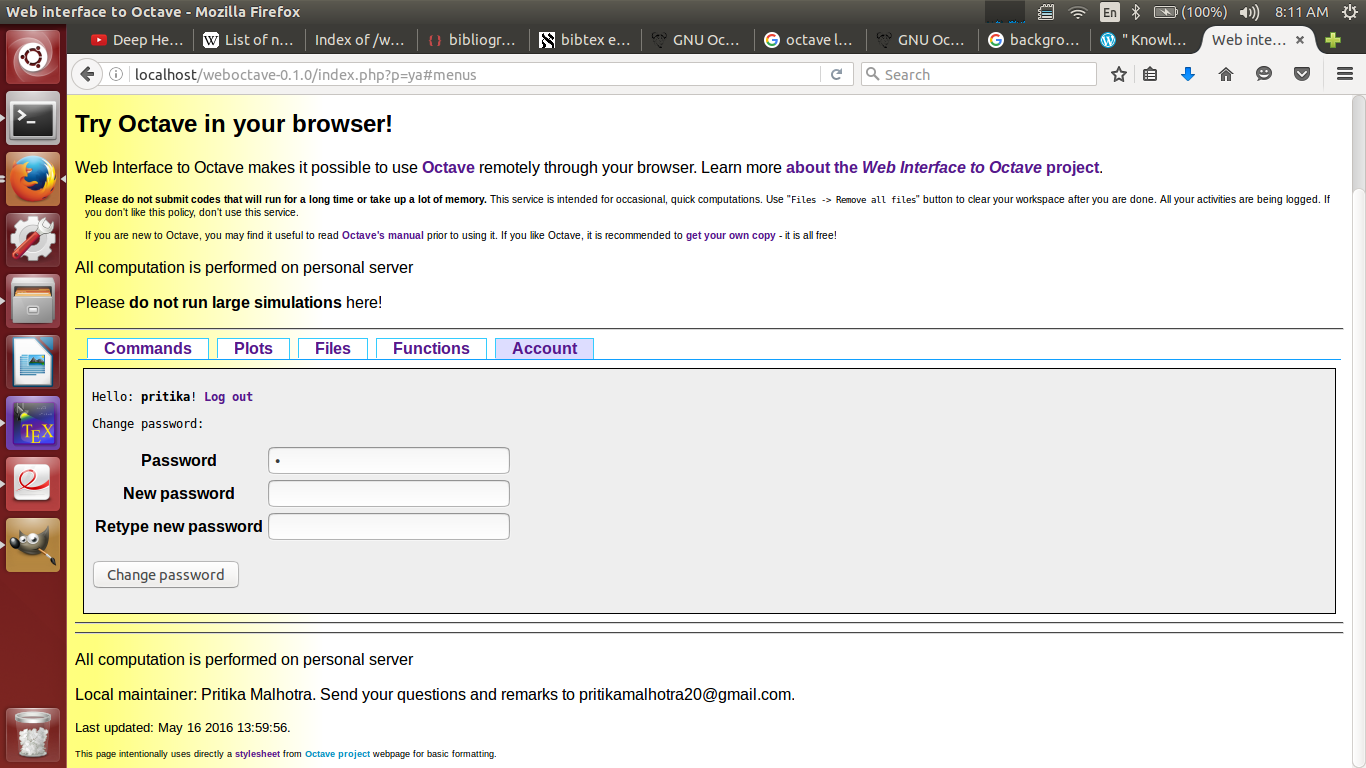
\includegraphics[width=0.7\textwidth]{images/account.png}                
 	\caption{Mesh}
 	\hspace{-1.5em}
 \end{figure}
 
 
 
 
 